\documentclass{article}
\usepackage{graphicx}
\usepackage[italian]{babel}
\usepackage{pdfpages}
\usepackage[utf8]{inputenc}
\usepackage[a4paper, total={6.5in, 8in}]{geometry}
\usepackage{listings}
\usepackage{hyperref}

\lstset{
  language=bash,
  basicstyle=\ttfamily
}
\setcounter{tocdepth}{2}

\title{Relazione Sistemi Operativi 2019/20} 
\author{Vannella Alessio}
\date{}
\begin{document}
\maketitle
\tableofcontents
\begin{abstract}
Questa breve relazione spiega le scelte progettuali attuate per la realizzazione del progetto didattico del corso di Sistemi Operativi dell'università di Torino. 
\end{abstract}
\section{Esecuzione e compilazione del codice} 
Per la compilazione del progetto è stato predisposto un makefile nella directory principale che compila tutte le dipendenze. In particolare, questi sono i modi di utilizzo: 
\begin{itemize}
    \item "make all": Compila senza eseguire nulla; 
    \item "make run": Compila ed esegue automaticamente il codice;
    \item "make clean": Pulisce tutti i file generati;
\end{itemize}
Il file di output eseguibile è denominato "game".\\Per impostare la modalità di gioco tra "easy" e "hard", nella sotto cartella config è presente un file bash "set\_cfg" che può essere richiamato con la sintassi:\\ 
\begin{center}
\begin{tabular}{c}
\begin{lstlisting}
./set_cfg mode
\end{lstlisting}
\end{tabular}
\end{center}

dove mode può assumere il valore di "easy" o "hard".




\section{Struttura del codice}
Il progetto è diviso diviso in moduli. Ogni modulo ha una funzione specifica per il progetto.\\Dal punto di vista strutturale, nella cartella "lib" sono presenti tutti gli header dei moduli, mentre nella cartella "src" sono presenti le definizioni di tutte le funzioni, diviso per moduli.\\I moduli sono divisi in due macro categorie: \textbf{librerie di gioco} e \textbf{librerie generiche}.

\subsection{Position}
La libreria position definisce l'omonimo tipo che  serve ad identificare univocamente una posizione sulla scacchiera.\\ Gli unici campi della struttura sono due interi x ed y, che indicano le due coordinate della posizione nella scacchiera.

\subsection{Cella}
La libreria cella definisce e si occupa di gestire le celle della scacchiera. Per farlo, definisce più tipi di dato: 
\begin{itemize}
    \item flag: utilizzata per rappresentare le bandiere sulla scacchiera;
    \item pawn: utilizzata per rappresentare le pedina sulla scacchiera;
    \item cella: la struttura che incapsula le due precedenti. Ogni cella può essere sia una pedina che una bandiera a seconda di come è inizializzata;
\end{itemize}

\subsection{Player}
La libreria player racchiude i comportamenti dei giocatori. Definisce una struttura player che ha come campi un intero che segna il numero del giocatore e un puntatore ad array di celle che salva un riferimento per ogni pedina di quel giocatore.\newline L'unica funzione definita serve a calcolare ed assegnare le indicazioni dal player alle proprie pedine.

\subsection{Scacchiera}
La libreria scacchiera raggruppa tutti gli strumenti utili per la gestione della scacchiera. Al suo interno è presente, oltre che una matrice di celle per rappresentare la scacchiera stessa, un vettore di celle per salvare le bandierine piazzate nella scacchiera e un intero che tiene traccia del numero delle bandierine rimaste in gioco.

\subsection{Statistics}
La libreria statistics è un contenitore logico per salvare le statistiche di gioco round dopo round.

\subsection{masterStruct}
La struttura masterStruct incapsula tutte le altre strutture definite precedentemente. Attraverso una variabile di tipo masterStruct si ha accesso a tutti gli elementi di gioco. 

\subsection{myIPC}
La libreria myIPC racchiude tutti gli strumenti per la sincronizzazione tra processi utilizzati nel progetto: semafori, code di messaggi e memoria condivisa. Inoltre, questa libreria definisce una struttura nella quale vengono salvati tutti gli id delle ipc utilizzate nel programma.

\subsection{genericLib}
La libreria genericLib definisce dei metodi che non hanno uno scopo preciso e serve anche ad interfacciare il codice principale con le varie librerie.
\section{Strategie adottate}

\subsection{Posizionamento delle pedine}
In fase di posizionamento delle pedine, la scacchiera è idealmente divisa in 8 sezioni isolate tra di loro. All'interno di ogni sezione c'è un numero definito di pedine per ogni giocatore. Ogni giocatore avrà almeno una pedina all'interno di ogni sezione. \newline Questo meccanismo permette di avere un numero equo di pedine sparse per tutta la scacchiera.
\subsection{Movimento delle pedine}
Prima dell'inizio del round, i giocatori calcolano la posizione della propria pedina più vicina ad ogni bandiera e ne impostano il target. \newline Una volta avviato il round, le pedine che hanno un target si muoveranno verso il loro l'obiettivo.\newline Le pedine restanti, invece, calcoleranno in modo dinamico la bandiera più vicina a loro e, se esiste, imposteranno il target su di essa e si muoveranno per conquistarla.
\\\\ Le pedine con un target, una volta conquistato il loro target (da parte loro o di pedine di altre squadre), si comporteranno come delle pedine senza target e cercheranno la bandiera più vicina alla loro posizione.\newline
I movimenti delle pedine sono limitati al quadrante nel quale sono state create. \\\\
Requisito fondamentale trovare un target è che la distanza tra la bandierina e la pedina sia minore o uguale a MAX\_DISTANCE, variabile calcolata in base ai parametri del gioco. Se questo requisito non è soddisfatto, le pedine resteranno ferme nella loro posizione per il round attuale.

\subsection{Comunicazione tra processi}
La comunicazione tra processi è realizzata utilizzando diversi strumenti di sincronizzazione. \newline
Lo stato della partita e i dati di gioco, sono salvati in memoria condivisa. Per realizzare questo meccanismo, sono state create diverse aree di memoria condivisa, una per un'intera struttura masterStruct e una per ogni array dinamico utilizzato nell'esecuzione del codice. \newline
Per segnalare al master che una bandiera è stata catturata, si utilizza una coda di messaggi che invia un messaggio al master con la posizione della bandiera da rimuovere e l'indice del giocatore che ha conquistato la bandiera.\\
Per quanto riguarda la sincronizzazione tra i vari gruppi di processi, si utilizzano dei semafori.\newline
I semafori invece sono utilizzati per eseguire l'accesso in mutua esclusione ai dati presenti nella memoria condivisa, per evitare l'accesso a dati inconsistenti. L'utilizzo dei semafori è fatto con il flag IPC\_NOWAIT.\newline
\begin{center}
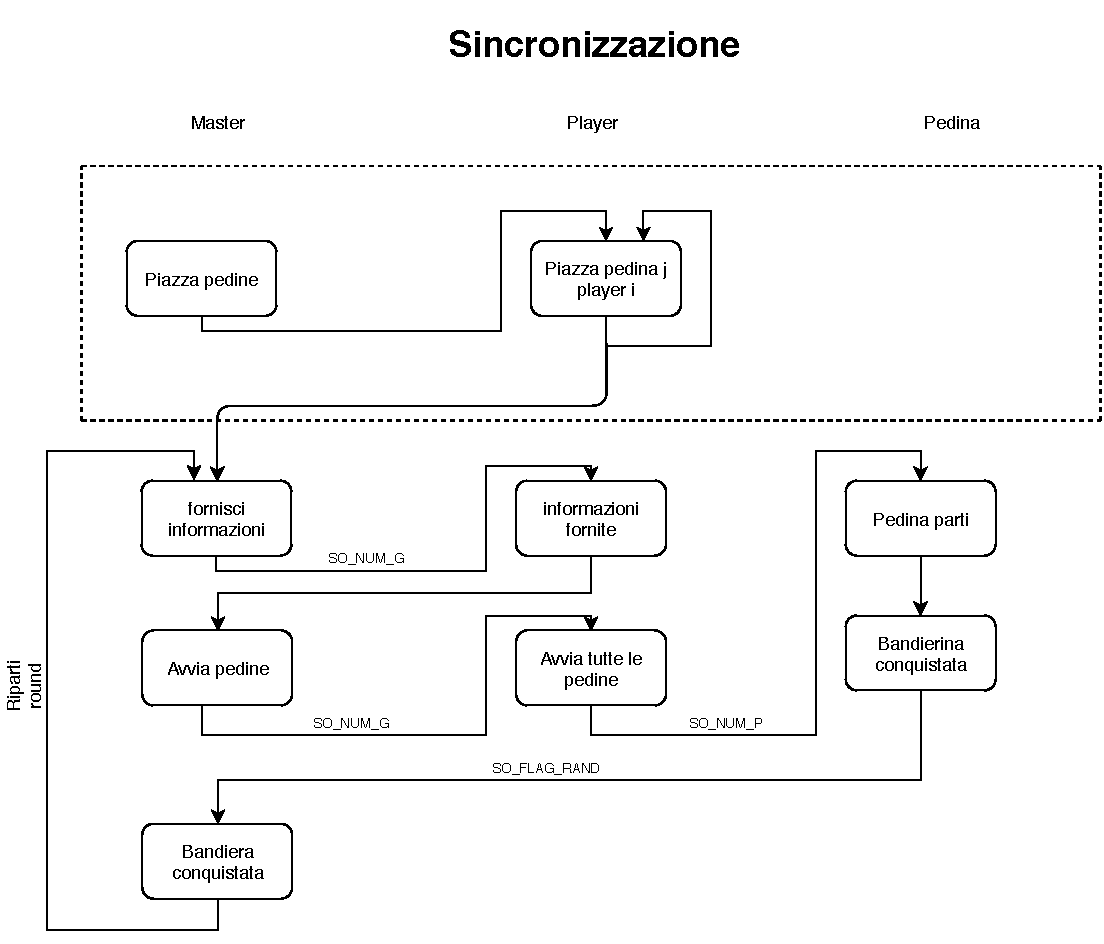
\includegraphics[width=.8\textwidth]{Sync.pdf}
\end{center}
\end{document}
